\chapter{Related Work}
\label{Chapter:RelatedWork}

To understand how software project telemetry relates to other research, it is useful to think in terms of two concepts: \textit{measurement machinery} and \textit{process methodology}. Measurement machinery refers to how software metrics are collected and analyzed. In software project telemetry, sensors collect metrics automatically and unobtrusively. Metrics are abstracted into telemetry streams, charts, and reports, representing high-level perspectives on software development. Project management and process improvement decisions are based on the trends in telemetry streams. Process methodology refers to specific techniques used to improve the quality of software development effort. Software project telemetry employs cycles of process problem detection, improvement hypothesis generation, change implementation, and hypothesis validation to empirically guide project management and process improvement decision-making.

This chapter compares and contrasts software project telemetry to other metrics-based approaches. Some approaches, such as the Personal Software Process (PSP) \cite{Humphrey:1995, Humphrey:1996}, can be compared to software project telemetry with respect to both measurement machinery and process methodology. Other approaches, such as the Constructive Cost Model (COCOMO)  \cite{Cocomo:1981, Cocomo:2000}, are only comparable with respect to measurement machinery. Still others, such as the Goal-Quality-Metric paradigm (GQM) \cite{Basili:1988, Basili:1992}, and the Software Capability Maturity Model (CMM) \cite{Paulk:1993, SEI:1995}, are only comparable with respect to process methodology. 


This chapter proceeds with an overview of software measurement theory in Section \ref{RelatedWork:MeasurementOverview}, which serve as the foundation for any software measurement programs.
Section \ref{RelatedWork:PSP} discusses the Personal Software Process. 
Section \ref{RelatedWork:COCOMO} discusses process prediction models, especially the Constructive Cost Model. 
Section \ref{RelatedWork:GQM} discusses the Goal-Question-Metric paradigm.
Section \ref{RelatedWork:CMM} discusses maturity frameworks, especially the Software Capability Maturity Model.
Section \ref{RelatedWork:Summary} concludes the chapter with a summary.




%%%%%%%%%%%%%%%%%%%%%%%%%%%%%%%%%%%%%%%%%%%%%%%%%%%%%%%%%
%                                                       %
%                   S E C T I O N                       %
%                                                       %
%%%%%%%%%%%%%%%%%%%%%%%%%%%%%%%%%%%%%%%%%%%%%%%%%%%%%%%%%

\section{Software Measurement Theory}  \label{RelatedWork:MeasurementOverview}

As noted by DeMarco \cite{DeMarco:1982}: \textit{``You can neither predict nor control what you cannot measure.''} Measurement is the first step to transform software engineering from an art where the success of a project depends largely on the competence and commitment of individual developer, to a scientific discipline where project outcome is both predictable and controllable.

Measurement is defined as the process by which numbers or symbols are assigned to attributes of entities in the real world in such a way as to describe them according to clearly defined rules \cite{Fenton:1997}. This definition depends on two related concepts: entity and attribute. 
An entity can be a physical object such as a program, an event such as a release milestone, and an action such as testing software. In software measurement, entities are usually divided into two categories: software product and process. 
An attribute is a property of an entity, such as the size of a program, the size of test scripts, and the time required to finish a milestone. Attributes are generally divided into two categories: internal and external. Measures for internal attributes can be computed based on the entity itself; while measures for external attributes depend on both the entity and the environment in which the entity resides. 
The resulting classification scheme is depicted in Table \ref{table:Software-Measurement-Classification}. The cell for internal software process attributes is empty, because all software process metrics are dependent on the environment to various degrees.

\begin{table}[tbp]
	\centering
		\caption{Software Measurement Classification}
		\begin{tabular}{|p{0.30\textwidth}|p{0.30\textwidth}|p{0.30\textwidth}|} 
			\hline
			{} & \textbf{Internal Attributes} & \textbf{External Attributes} \\
			\hline
			\textbf{Software Product} & size, complexity, cohesion, coupling, etc. & quality, reliability, maintainability, portability, etc. %\cite{Musa:1987}
			\\
			\hline
			\textbf{Software Process} & {} & time, effort, cost, etc. \\
			\hline
		\end{tabular}
	\label{table:Software-Measurement-Classification}
\end{table}


The representation theory of measurement formalizes the process of mapping from an empirical relation system to a numerical relation system. A ``measure'' is nothing but the number assigned to describe some attribute of an entity by the mapping process. Not all mappings are the same. For example, the result of a sports competition, the first place, the second place, and the third place, are usually mapped to real numbers \textit{1}, \textit{2}, and \textit{3}, respectively. Since sports competition results contain only ordinal information, it is equally valid to use \textit{1}, \textit{10}, and \textit{100} as the mapping result. It is meaningless to add these numbers. This simple example shows that not all valid mathematical analyses in a numerical relation system are valid in the original empirical relation system.

Formally, the mapping, together with the associated empirical and numerical relation systems, is called the \textit{``measurement scale.''} It is the measurement scale that determines valid mathematical operations that can be performed. In general, measurement scales are classified into four categories with increasing level of restrictiveness: nominal, ordinal, interval, and ratio. More restrictiveness means more mathematical operators in the numerical relation system can be applied. Table \ref{table:MeasurementScaleAndOperator} lists the types of measurement scale and their corresponding valid mathematical operators.

\begin{table}[tbp]
	\centering
		\caption{Measurement Scale and Valid Mathematical Operations}
		\begin{tabular}{|p{0.45\textwidth}|p{0.45\textwidth}|} 
			\hline
			\textbf{Measurement Scale} & \textbf{Valid Mathematical Operators} \\
			\hline
			{Nominal Scale} & $=$ \\
			\hline
			{Ordinal Scale} & $=$ $>$ $<$ \\
			\hline
			{Interval Scale} & $=$ $>$ $<$ $+$ $-$ \\
			\hline
			{Ratio Scale} & $=$ $>$ $<$ $+$ $-$ $*$ $/$\\
			\hline
		\end{tabular}
	\label{table:MeasurementScaleAndOperator}
\end{table}

\begin{itemize}
	\item \textbf{Nominal Scale} --- The empirical relation system consists only of different classes. An example is the type of software fault, such as specification, design, and coding. There is no notion of ordering between different classes. As a result, any distinct number representation is a valid measure.
	
	\item \textbf{Ordinal Scale} --- It preserves ordering. The empirical relation system consists of classes that are ordered. An example is defect severity, such as minor, major, and critical. Any mapping that preserves the ordering is a valid mapping, and the numbers represent ranking only. Arithmetic operations, such as addition, subtraction, multiplication, and division, have no meaning.
	
	\item \textbf{Interval Scale} --- It preserves not only ordering but also differences. The difference between any two of the ordered classes in the range of the mapping is the same. Only addition and subtraction are valid. For example, when talking about time, we can say that ``year 2000 is 1000 years later than year 1000,'' and ``year 3000 is 1000 years later than year 2000,'' but we cannot say that ``year 2000 is twice as late as year 1000.'' 
	
	\item \textbf{Ratio Scale} --- It preserves ordering, differences, and ratios. The measurement starts from a zero element representing total lack of attribute, and increases at equal intervals known as units. All arithmetic operations, addition, subtraction, multiplication, and division, can be meaningfully applied. Using the length of software code as an example, we can say that ``this code contains no line,'' ``this code contains 20 more lines than that code,'' and ``this code contains twice as many lines as that code.''

\end{itemize}


 

In the current implementation of software project telemetry, mathematical computation of software metrics occurs at two consecutive stages: reduction processing and telemetry language processing. 

Reduction processing is the process of generating basic telemetry streams by filtering, synthesizing, and aggregating raw metrics collected by sensors. Telemetry reducers implement different reduction behaviors. They form the lowest level, atomic ``building blocks'' of the software project telemetry observable by an end user. Though data points in telemetry streams are mapped to real numbers by the reduction process, they can be of any measurement scale in theory. The reduction process itself is treated as a black box by the telemetry infrastructure. This is not a problem to end users, because the internal implementation details of telemetry reducers are not exposed to them. However, the developers who are responsible for reducer implementation must make sure that sensor data are manipulated in a meaningful way.

Telemetry language processing acts on telemetry streams. It includes telemetry function calls and telemetry arithmetic operations. The data points in telemetry streams are treated as if they were of ratio scale by the language interpreter. As a result, the language allows addition, subtraction, multiplication, and division between telemetry streams. This might cause a problem to a careless user, because there is the theoretical possibility of scale type mismatch. In other words, the telemetry language might allow meaningless mathematical operations to be applied to different types of metrics, such as adding code churn metric to unit test coverage metric. The problem could be solved by introducing a ``type'' system to the language, but doing so would significantly complicate the language design and its implementation. Currently, software project telemetry takes a pragmatic approach by relying on the user defining telemetry constructs to recognize nonsense operations. A topic for future research is to determine whether scale type mismatch is a significant problem in the use of software project telemetry, and to devise appropriate mechanisms to detect and/or prevent this problem.








%%%%%%%%%%%%%%%%%%%%%%%%%%%%%%%%%%%%%%%%%%%%%%%%%%%%%%%%%
%                                                       %
%                   S E C T I O N                       %
%                                                       %
%%%%%%%%%%%%%%%%%%%%%%%%%%%%%%%%%%%%%%%%%%%%%%%%%%%%%%%%%

\section{Personal Software Process}  \label{RelatedWork:PSP}

The Personal Software Process (PSP\footnote{Both Personal Software Process and PSP are registered service marks of Carnegie Mellon University.}) \cite{Humphrey:1995, Humphrey:1996} is a self-improvement process for software developers, and a ground-breaking approach that adapts organizational-level software measurement and analysis techniques to individuals. 

The PSP provides both measurement machinery and process methodology. The primary goal of the PSP is to improve project estimation and quality assurance. The goal is pursued by observation-evaluation-modification cycles. Developers observe their performance by recording how they develop software. They record the amount of time they spend, the size of the work product, and the defects they make while developing software. At the end of each project, developers evaluate how they performed by conducting standard analyses on the metrics they collected. Based on project postmortems, developers gain insight into their development process, and modify it in an attempt to improve it. A new cycle starts with the modified development process.

The original PSP proposed by Humphrey uses the very tedious manual approach to collect and analyze metrics. For instance, every time a compilation error occurs, the developer has to stop his/her current work, and log on paper forms the details of the error. Though several studies \cite{Ferguson:1997, Hayes:1997, Khajenoori:1995} have shown that the PSP appears to help improve software development, the anecdotal evidence suggests that the overhead involved in manual data collection affects its adoption. For example, a report on a workshop of PSP instructors \cite{Borstler:2002} reveals that in one course of 78 students, 72 of them abandoned the PSP because they felt \textit{``it would impose an excessively strict process on them and that the extra work would not pay off.''} None of the remaining 6 students reported any perceived process improvements. Moreover, manual data collection is susceptible to bias (either deliberate or unconscious), error, omission, and delay. A study \cite{Johnson:1998} of the data collected in the PSP showed that there were significant issues of data quality, and the combination of data collection and analysis errors called into question the accuracy of manual PSP results. Humphrey, the author of PSP, also admits in his book ``A Discipline for Software Engineering'' \cite{Humphrey:1995} that \textit{``it would be nice to have a tool to automatically gather the PSP data.''}

Tools, such as LEAP \cite{Moore:1999}, PSP Studio \cite{PspStudio:1997} and Software Process Dashboard \cite{PspDashboard:2000}, do exist to support the original manual PSP. These tools follow the same approach to user interaction by displaying dialog boxes where the user can log effort, size, and defect information. Though tool support lowers data collection overhead considerably, it turns out that the adoption of these tools is not satisfactory because of the requirement that the user constantly switch back and forth between doing work and telling the tool what work is being done \cite{Johnson:2001, Johnson:2003}. This chronic context switch appears to be a problem for many developers.

Software project telemetry uses sensors to collect metrics.\footnote{Sensor-based approach to metrics collection is pioneered in the Hackystat project \cite{Johnson:2003}, developed in the Collaborative Software Development Lab at University of Hawaii. I have been on the Hackystat development team since 2002 while doing software project telemetry research.} Sensors are attached to software development tools, which monitor some form of state change in the project development environment. Sensors collect metrics automatically and unobtrusively so that developers are not distracted from their primary tasks -- developing software products. Compared to manual and tool-based metrics collection, the sensor-based approach not only automates metrics collection in an unobtrusive manner, but also eliminates the chronic context-switch overhead. Details about sensor data collection, along with its restrictions, are discussed in Section \ref{Telemetry:Data}.

With respect to process methodology, the PSP uses observation-evaluation-modification cycles to improve software development process. One cycle corresponds to the life time of a project, and process improvement is based on comparison of different projects. This is essentially model-based cross-project comparison. The limitation is that it requires a historical database of finished projects. The PSP does not yield benefit unless such a database is accumulated first. For example, one of the practices of the PSP is to use statistical regression to predict project time based on planned project size, which requires a sufficient number of data points with respect to time and size of the past projects. Even if the accumulation of a historical project database is not a problem, the PSP user still must make sure that the context of the current project is consistent with the contexts of the finished projects in the project database. Otherwise, the prediction process is like comparing apples to oranges. The context consistency problem will be discussed in detail in Section \ref{RelatedWork:COCOMO}, since all model-based approaches face the same limitation.

Similar to the PSP, software project telemetry uses cycles to improve the software development process. The cycle includes process problem detection, hypothesis generation, change implementation, and hypothesis validation. The difference is that a software project telemetry cycle does not correspond to the life time of a project. It involves much smaller time scale, and a single project typically has many cycles. The idea is that comparisons can be made between two different periods of the same project instead of between two different projects, and that the changes in the development process and their trends can be used as the basis for decision-making in project management and process improvement. Since software project telemetry does not make model-based cross-project comparisons, there is neither a need to accumulate a historical project database, nor a necessity to ensure context consistency between different projects.







%%%%%%%%%%%%%%%%%%%%%%%%%%%%%%%%%%%%%%%%%%%%%%%%%%%%%%%%%
%                                                       %
%                   S E C T I O N                       %
%                                                       %
%%%%%%%%%%%%%%%%%%%%%%%%%%%%%%%%%%%%%%%%%%%%%%%%%%%%%%%%%

\section{Constructive Cost Model and Model-based Process Predictions} \label{RelatedWork:COCOMO}

The Constructive Cost Model (COCOMO) \cite{Cocomo:1981, Cocomo:2000} is a model for software project cost / effort estimation. It belongs to the branch of software engineering research called \textit{model-based process prediction}. This section begins with the more general topic of model-based process prediction before going into the details of the COCOMO.

The research in the area of model-based process prediction typically involves the following basic procedure: (1) collect a set of process and product metrics, such as size, effort, complexity, and defects, for a set of completed software projects, (2) generate a model to fit the observed data, (3) and claim that the model can be used to predict characteristics of future projects. For example, a model might predict that a future project of size \textit{S} will require \textit{E} person-months of effort; another model might predict that the future implementation of a module with complexity \textit{C} will be prone to defects with density \textit{D}. 

Model-based process prediction can be compared to software project telemetry with respect to measurement machinery. The difference is that prediction in software project telemetry does not require model building. Instead, it relies on changes in the development process and their trends to make short-term in-process predictions. The predictions made in software project telemetry and those made in model-based approaches tend to be of a different nature: model-based approaches tend to make end-point estimations (i.e., predictions for all phases of a software project as a whole), such as $X$ man-hours are needed to finish project $A$; while software project telemetry tends to make in-process predictions, such as the number of open bugs in system $B$ will continue to increase if system test coverage does not stop dropping.

Since model-based process prediction follows similar approaches in model building and process prediction, COCOMO is used to illustrate how they work in general. COCOMO is chosen because it is one of the most widely available and accepted models in the public domain.
%The Constructive Cost Model (COCOMO) \cite{Cocomo:1981, Cocomo:2000}
It is developed by Barry Boehm and his associates at University of Southern California.  The model estimates effort and schedule required to complete a software project. COCOMO 81 was the original model published in the book \textit{Software Engineering Economics} \cite{Cocomo:1981}. It offers three levels of model with increasing detail and accuracy: basic, intermediate, and detailed. COCOMO II \cite{Cocomo:2000} is an updated version of the original model to reflect the changes in software development practice. Like the first version, COCOMO II offers three levels: application composition, early design, and post-architecture, to explicitly model the fact that uncertainty of effort and schedule estimates decreases through software project life cycle. 

The post-architecture model is used to illustrate how COCOMO works. The estimation equations in the post-architectural model are:
  \begin{equation}
    PM = A * \prod_{i=1}^{17}EM_{i} * Size ^{(B + 0.01 * \sum_{i=1}^{5}SF_{i})}
  \end{equation}

  \begin{equation}
    TDEV = C * PM ^{(D + 0.002 * \sum_{i=1}^{5}SF_{i})}
  \end{equation}
where $PM$ is estimated effort in person-months. A person-month is the amount of time one person spends working on a software development project for one month. Note that this is in nominal terms, which does not take schedule compression or expansion into account.\footnote{COCOMO II offers an effort multiplier $SCED$, which can be used to adjust for the effect of schedule compression or expansion.} $Size$ is the primary input to the model. It is expressed in thousands of source lines of code (KSLOC). COCOMO II not only offers detailed rules on how to count lines of code, but also provides methods to convert other counting results, such as function points\footnote{A function point is a measure of program size independent of technology and programming language. The value of function point $FP$ is the product of unadjusted function point $UFP$ and technical correction factor $TCF$. Support for setting up function point analysis program is available from International Function Point User Group (http://www.ifpug.org).} \cite{Albrecht:1983} and object points \cite{Banker:1991, Banker:1994}, to lines of code. $TDEV$ is the amount of calendar time it will take to develop the software product. The average number of staff can be derived by dividing $TDEV$ from $PM$.

$A$, $B$, $C$, $D$, $SF_i$ and $EM_i$ are all constants in the model. $SF_i$ is called scale factor which influences effort exponentially. Scale factors are used to account for the relative economy or dis-economy of scale encountered for software projects of different sizes. $EM_i$ is called effort multiplier which influences effort multiplicatively. Effort multipliers are used to adjust for different product, project, platform and personnel factors in different software product development. Both effort multipliers and scale factors are defined by a set of rating levels: \textit{Very Low}, \textit{Low}, \textit{Nominal}, \textit{High}, \textit{etc}. 

Every few years, the COCOMO team updates the model by supplying new calibration values for the constants to reflect latest change in software production practice in industry. For example, the calibration values for the COCOMO II 2000 post-architecture model were obtained by calibrating the model to the actual parameters and effort values for the 161 projects in the COCOMO II database at that time. These values represent the software industry average. COCOMO recommends its users to calibrate $A$, $B$, $C$ and $D$ to their local development environment in order to increase prediction accuracy of the model.

COCOMO enjoys wide acceptance in both academia and industry. Various extensions have been developed since the publication of the original model. These extensions include COQUALMO (Constructive Quality Model) \cite{COQUALMO:1999}, COCOTS (Constructive COTS Model) \cite{COCOTS:2000}, and CORADMO (Constructive Rapid Application Development Model) \cite{CORADMO:2001}. Commercial implementations include Costar from Softstart Systems \cite{Software:Costar}, Cost Xpert from Cost Xpert Group Incorporated \cite{Software:CostXpert}, and Estimate Professional from Software Productivity Center Incorporated \cite{Software:EstimateProfessional}. 

The basic idea behind COCOMO and other process prediction models is ``cross-project comparison.'' Unfortunately, there are a number of difficulties in adopting this method in practice.

First, model-based process prediction assumes that the software organization has a relatively stable and repeatable development process. However, according to a Software Engineering Institute (SEI) survey of 542 software development organizations \cite{Peterson:1997}, 67\% of them are at CMM Level 1: the lowest maturity level. By definition, the software processes at level 1 are \textit{ad hoc} and sometimes \textit{chaotic}, and they change as work changes. As a result, it is generally impossible to make predictions for organizations at this level. In other words, two-thirds of software organizations are incapable of benefiting from model-based process predition techniques, such as COCOMO.

Second, the prediction power of these models is highly dependent on how well model calibration is performed. This can be thought of as a context consistency problem. In order to use the model, practitioners must confirm that the set of projects used to calibrate the model are similar to the project they wish to predict. Otherwise, they must recalibrate the model using the data in the organization's historical project database. This involves replicating the model-building method within the practitioner's organization, with the risk that the organization may have already changed and the context of the current project may differ from those in the historical project database, not to mention the practicality and cost of accumulating such a historical project database in the first place. 

Lastly, model-based process predictions are primarily designed to be used at a very early stage of a software project, or even before a project actually starts. Therefore, they tend to make end-point estimations (i.e., the prediction is made for all phases of the project as a whole). For example, COCOMO estimates that 586 person-months are required to develop a software with estimated size of 100 KSLOC.\footnote{Suppose all scale factors and effort multipliers take the rating of \textit{nominal}. Using COCOMO II 1997 calibration data, the estimation equation is $PM = 2.94 * Size ^ {1.15}$.} But when 300 person-months have been spent writing 60 KSLOC, the model does not give any indication whether the project will still be on-target or not. The project manager will know the answer after the entire project is finished, but by that time the information is irrelevant. To put it simply, end-point estimation is not very effective for in-process control.

Software project telemetry avoids the above-mentioned difficulties by shifting the focus of process prediction. It makes no attempt to build a cross-project comparison model in order to make a prediction before the project starts. Instead, it employs a more agile approach to compare software processes in different periods within the same project. It relies on changes in software development process and the trends of those changes to make short-term predictions for the purpose of in-process project management. 










%%%%%%%%%%%%%%%%%%%%%%%%%%%%%%%%%%%%%%%%%%%%%%%%%%%%%%%%%
%                                                       %
%                   S E C T I O N                       %
%                                                       %
%%%%%%%%%%%%%%%%%%%%%%%%%%%%%%%%%%%%%%%%%%%%%%%%%%%%%%%%%

\section{Goal-Question-Metric Paradigm} \label{RelatedWork:GQM}

The Goal-Question-Metric paradigm (GQM) \cite{Basili:1988, Basili:1992} provides a top-down, goal-oriented process methodology: software measurement is driven by high level goals. Usually the business goals of an organization are formed first, and then translated into improvement goals of software development, which, in turn, are translated into measurement goals. A metrics program is used to fulfill these measurement goals. Based on the measurement results, the organization can generate hypotheses and make decisions to reach the software development improvement goals, and, finally, the business goals.

GQM measurement goal is stated in 5 dimensions: \textit{study object}, \textit{purpose}, \textit{quality focus}, \textit{view point}, and \textit{environment}. A concrete example can be found in \cite{Solingen:1998, Solingen:1999}, in which the authors studied causes and effects of interruptions on software development work, and their measurement goal was:

\begin{quote}	
 \textit{Analyze} interrupts and their effects \textit{for the purpose of} understanding \textit{with respect to} impact on schedule and the cost-benefit of interrupts \textit{from the viewpoint of} project team \textit{in the context of} project $X$.
\end{quote}

GQM includes a top-down methodology that translates measurement goals into questions that need to be answered in order to reach them. Based on the questions, a set of relevant metrics can be identified and collected, which provide answers to the questions. The methodology can be best visualized as a tree-structured graph in Figure \ref{fig:gqm}.

\begin{figure}[tbp]
	\centering
		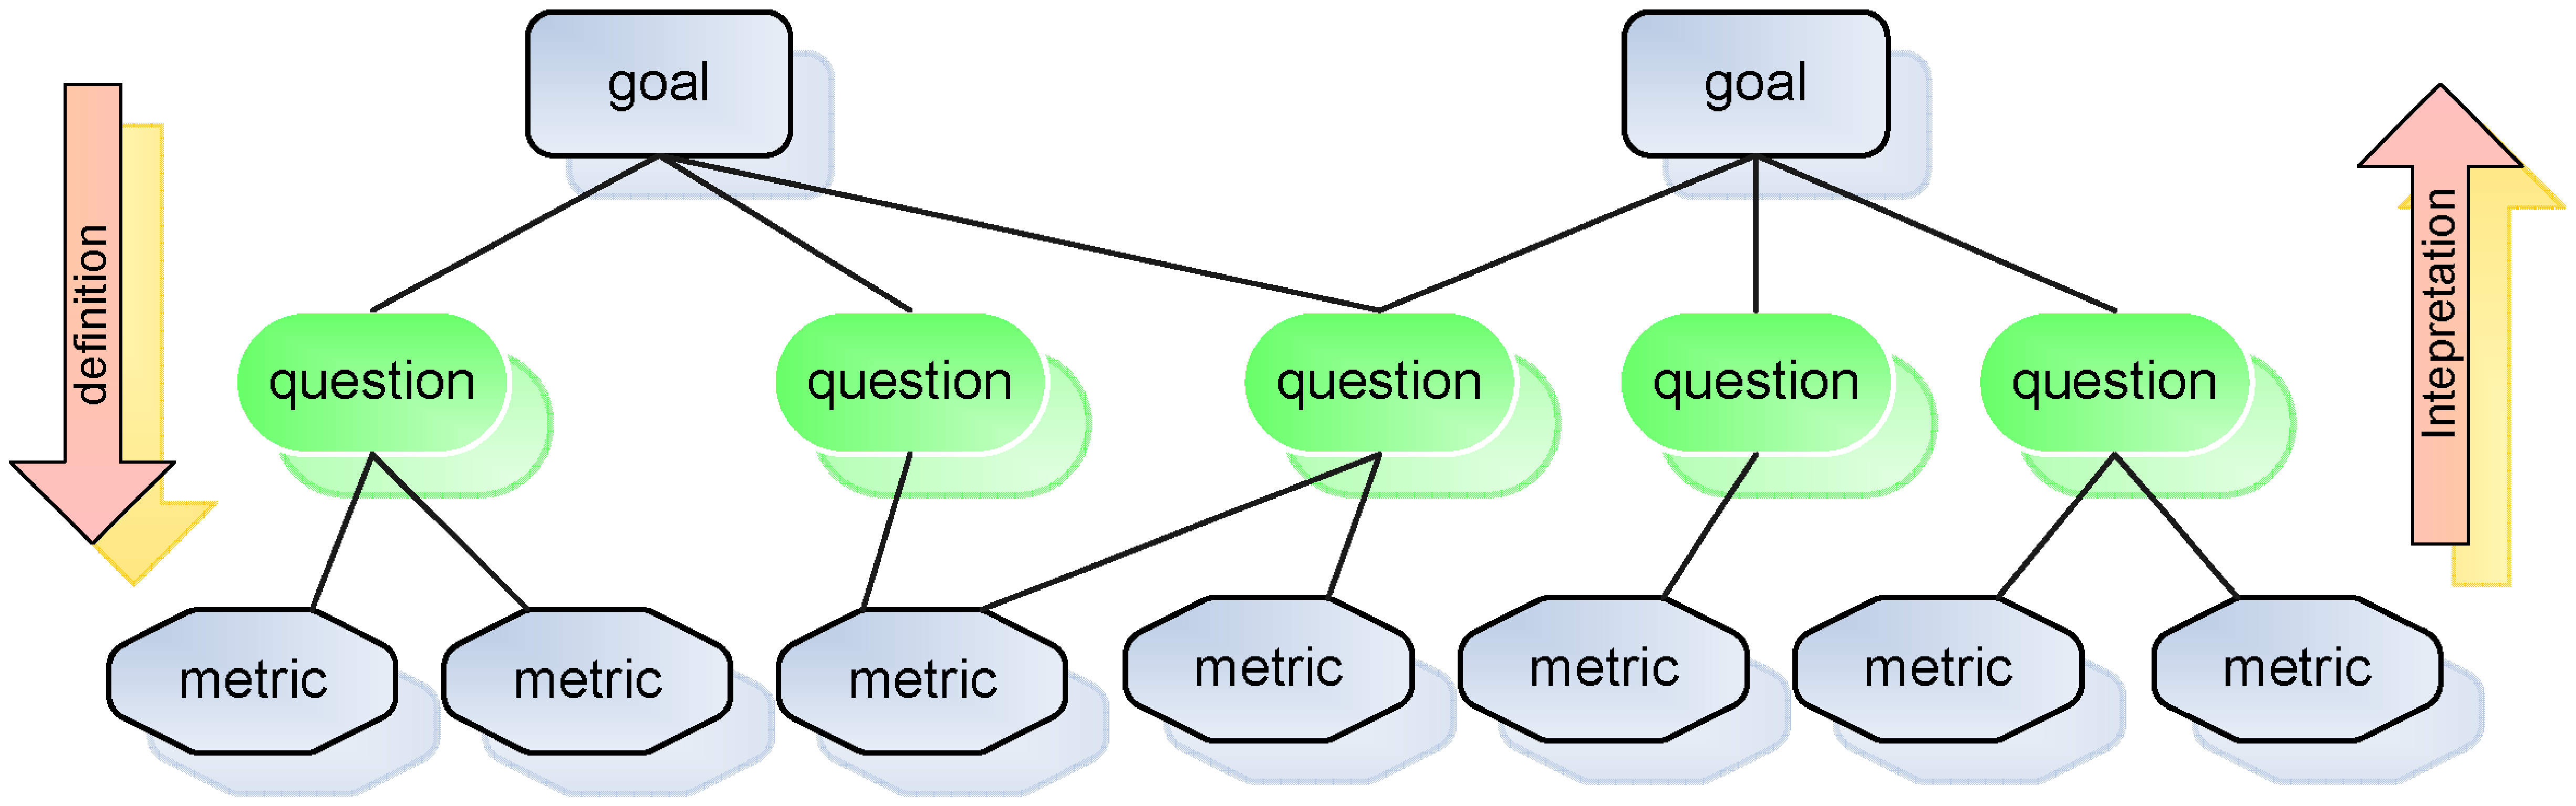
\includegraphics[width=1.00\textwidth]{figures/GQM}
		\caption{Goal-Question-Metric Paradigm}
	\label{fig:gqm}
\end{figure}

The GQM paradigm is well-known, and case studies of successful experience abound \cite{Basili:1996, Latum:1998, Fuggetta:1998}. The key to a success GQM implementation appears to be the establishment of well-defined measurement goals and the derivation of software metrics that can be used to provide useful information to meet the goals. However, the main criticism of GQM is the lack of attention to the actual measurement process: metrics collection and interpretation are not part of the paradigm. GQM implicitly assumes that once all required metrics are identified, the rest of the steps (metrics collection and interpretation) are easy.

Software project telemetry and the GQM paradigm can complement each other: GQM defines useful software metrics and relates them to an organization's business, project, product, and process goals; while software project telemetry provides an automated machinery for metrics collection and analysis. For example, ``Continuous GQM'' \cite{Lofi:2005} tries to implement GQM in an automated way in which data is collected, analyzed, and presented automatically with minimal human effort .








%%%%%%%%%%%%%%%%%%%%%%%%%%%%%%%%%%%%%%%%%%%%%%%%%%%%%%%%%
%                                                       %
%                   S E C T I O N                       %
%                                                       %
%%%%%%%%%%%%%%%%%%%%%%%%%%%%%%%%%%%%%%%%%%%%%%%%%%%%%%%%%

\section{Capability Maturity Model and Process Maturity Frameworks}  
\label{RelatedWork:CMM}

The Capability Maturity Model (CMM) \cite{Paulk:1993, SEI:1995} is a process maturity framework developed by the Software Engineering Institute (SEI). Other similar frameworks include ISO 9001 \cite{ISO9001:1987}, SPICE, and ISO/IEC 15504 \cite{ISO:1998, Eman:1998}. These frameworks share common properties, such as using metrics as a means to help software organizations improve their development process and to assess their capabilities. In these approaches, an externally defined reference framework is used to prescribe the activities, methodologies and practices a software organization should implement. The implicit assumption is that the prescribed processes are needed by most organizations in order to deliver high quality software in a repeatable and controllable manner, and a mature software development process will deliver high quality software products on time and within budget. Process assessment is used to compare organizational processes with the reference framework, which serves as an effective driver for process improvement. The assessment can be done by the software organization itself, by a second party, or by an independent third party. Based on the assessment results, organizations can find directions for process improvement.

Software project telemetry is closely related to process maturity. On the one hand, higher process maturity offers greater visibility into development activities. Since we can only measure what is visible in a process, higher process maturity means more telemetry streams can be generated and monitored. Process maturity frameworks offer a convenient context to plan software project telemetry program so that it grows to embrace additional aspects of software development and management. On the other hand, software project telemetry offers a methodology for process improvement based on quantitative feedback from existing development processes. It is especially helpful for software organizations to achieve high level process maturity where quantitative measurement is required.
Indeed, several authors have studied the relationship between software measurement and process maturity. For example, Table \ref{table:Maturity-Measurement} lists Pfleeger and McGowan's recommendation of collecting different measures depending on a software organization's CMM maturity level \cite{Pfleeger:1990}.

\begin{table}[tbp]
	\centering
		\caption{Process Maturity and Measurement}
		\begin{tabular}{|p{0.45\textwidth}|p{0.45\textwidth}|}
			\hline
			\textbf{CMM Maturity Level} & \textbf{What to Measure} \\
			\hline 
			\textit{Level 1 -- Initial: ad hoc} & baseline \\
			\hline 
			\textit{Level 2 -- Repeatable: process dependent on individual} & project \\
			\hline 
			\textit{Level 3 -- Defined: process defined and institutionalized} & product \\
			\hline 
			\textit{Level 4 -- Managed: process measured quantitatively} & process and feedback for control \\
			\hline 
			\textit{Level 5 -- Optimizing: continuing improvement based on measurement} & process and feedback for changing process \\
			\hline		
		\end{tabular}
	\label{table:Maturity-Measurement}
\end{table}

The following discussion uses CMM as an example to illustrate how a maturity framework works. Note that CMM is used here as a generic term referencing the works published by SEI, which include SW-CMM v1.0 (1991), SW-CMM v1.1 (1993), CMMI v1.02 (2000), and CMMI v1.1 (2002). CMMI \cite{Royce:2002} is the acronym for Capability Maturity Model Integration.

The goal of CMM is to determine whether a software development organization has a sound management infrastructure, and to assess its level of competence in building high quality software products. CMM is a staged model, which provides a set of requirements that software development organizations can use to set up software processes to control software product development. It ranks a software organization's process capability on a maturity level from 1 (lowest) to 5 (highest):

\begin{enumerate}
  \item \textbf{Initial Stage:} The software process at this level is characterized as \textit{ad hoc} and sometimes \textit{chaotic}. Success of software projects depends on the competence and commitment of individual developers. Few software processes are defined, and they change as work progresses. As a result, schedules, budgets and quality are generally unpredictable.
  \item \textbf{Repeatable Stage:} Basic project management processes are in place. Software organizations at this level have controls over software requirements, project planning and tracking, configuration management, quality assurance and subcontractor management. They are able to track project cost and schedule. They can repeat earlier successes on projects with similar applications.
  \item \textbf{Defined Stage:} The software processes for both management and engineering activities are documented, standardized and integrated into a standard software process for the whole organization. All projects use an approved, tailored version of the organization's standard software process to develop and maintain software.
  \item \textbf{Managed Stage:} Detailed measurement programs are in place to assess software development processes and product quality. Both software process and products are quantitatively understood and controlled. Software organizations at this level are able to tailor development processes to specific needs with predictable outcomes.
  \item \textbf{Optimizing Stage:} Continuous process improvement is enabled by quantitative feedback from software development processes and from piloting innovative ideas and technologies.
\end{enumerate}

Each maturity level is associated with a number of processes that an organization must implement. These processes are grouped into key process areas (KPA). Each KPA has a set of goals, capabilities, key practices, as well as measurements and verification practices. There are a total of 52 goals and 150 key practices. Some are related to setting up basic project management controls; some are aimed at establishing an infrastructure that institutionalizes effective software engineering and management processes across projects; while the rest are focused on performing a well-defined engineering process that integrates all software engineering activities to produce correct, consistent software products effectively and efficiently. The maturity level of a software organization is determined by its demonstrated capability in the key process areas associated with that level. Table \ref{table:CMM-KPA} lists CMM levels and their associated key process areas.

\begin{table}[tbp]
	\centering
		\caption{CMM Levels and Key Process Areas}
		\begin{tabular}{|p{0.25\textwidth}|p{0.65\textwidth}|} 
		  \hline
			\textbf{CMM Levels} & \textbf{Key Process Areas} \\
			\hline 
			\textit{Level 1 -- Initial} & None. \\
			\hline
			\textit{Level 2 -- Repeatable} & Requirements Management, Software Project Planning, Software Project Tracking and Oversight, Software Subcontract Management, Software Quality Assurance, Software Configuration Management. \\
			\hline
			\textit{Level 3 -- Defined} &  Organization Process Focus, Organization Process Definition, Training Program, Integrated Software Management, Software Product
Engineering, Intergroup Coordination, Peer Reviews. \\
			\hline
			\textit{Level 4 -- Managed} & Quantitative Process Management, Software Quality Management. \\
			\hline
			\textit{Level 5 -- Optimizing} & Defect Prevention, Technology Change Management, Process Change Management. \\
			\hline
		\end{tabular}
	\label{table:CMM-KPA}
\end{table}

CMM has received much attention in both academia and industry. Quite a few positive experiences have been reported in the literature \cite{Humphrey:1991, Dion:1993, Daskalantonakis:1994, Diaz:1997}. For example, Humphrey \textit{et. al. }\cite{Humphrey:1991} reported a software process improvement program at Hughes Aircraft with estimated annual saving at about \$2 million.

CMM makes use of software metrics to help software organizations improve their development process. It prescribes that in all key process areas measurement should be taken to determine the status of development activities. However, it does not prescribe how the measurement process itself should be implemented. In fact, Humphrey appears to be aware of the difficulty in implementing a measurement program in a software organization. He mentioned in \cite{SEI:1995} that:

\begin{quote}
\textit{``The greatest potential problem with the managed process is the cost of gathering data. There are an enormous number of potentially valuable measures of the software process, but such data is expensive to gather and to maintain.''}
\end{quote}
 
Software project telemetry can complement CMM. It provides not only an automatic and unobtrusive way of gathering software metrics data, but also a methodology of using quantitative data to analyze and modify software development process in order to prevent problems and improve efficiency. It is especially helpful for software organizations to achieve CMM Level 4 and 5.










%%%%%%%%%%%%%%%%%%%%%%%%%%%%%%%%%%%%%%%%%%%%%%%%%%%%%%%%%
%                                                       %
%                   S E C T I O N                       %
%                                                       %
%%%%%%%%%%%%%%%%%%%%%%%%%%%%%%%%%%%%%%%%%%%%%%%%%%%%%%%%%

\section{Chapter Summary}  \label{RelatedWork:Summary}

In this chapter, I have compared and contrasted Software Project Telemetry to other metrics-based approaches. The Personal Software Process suffers from chronic metrics collection and analysis overhead. The Constructive Cost Model relies on the assumption that software development process is stable and thus predictable. The Goal-Question-Metric paradigm offers a high-level abstract process methodology but lacks attention to the actual measurement process. The Capability Maturity Model prescribes that measurement should be taken to assess the status of development activities but does not specify how software measurement itself should be implemented. Software Project Telemetry addresses these limitations through automated metrics collection and analysis, and in-process, empirically-guided software development process problem detection and diagnosis. The next chapter gives a detailed discussion of Software Project Telemetry.

